\documentclass[aspectratio=169, 14pt]{beamer}
\usepackage[utf8]{inputenc}
\usepackage[english]{babel}
\usepackage{tipa}
\usepackage{graphicx}
\usepackage{transparent}
\usepackage[ruled, lined, linesnumbered, commentsnumbered]{algorithm2e}
\usepackage{pgfplots}
\newcommand\mycommfont[1]{\small\ttfamily\textcolor{blue}{#1}}
\SetCommentSty{mycommfont}
\renewcommand{\thealgocf}{}
\usepackage{setspace}
\usepackage{tikz}
\usetikzlibrary{matrix,backgrounds}
\usetikzlibrary{arrows}
\usetikzlibrary {arrows.meta}
\usetikzlibrary{calc,shadows.blur,fit,positioning}
\usetikzlibrary{shapes.multipart,chains}
\usepackage{minted}
\usepackage{fontawesome5}
\usepackage{booktabs}
\usepackage{caption}
\usepackage{bookmark}
\usepackage{hyperref}
\hypersetup{
    colorlinks=true,
    linkcolor=blue,
    filecolor=magenta,      
    urlcolor=cyan,
    }
\urlstyle{same}
\usetheme{metropolis}
\metroset{block=fill}
\usecolortheme{default}
\definecolor{darkmidnightblue}{rgb}{0.0, 0.2, 0.4}
\definecolor{LightGray}{gray}{0.9}

\definecolor{allcolor}{RGB}{148,182,233}
\newcommand*{\equal}{=}
\usepackage{pst-poker}
\usepackage[normalem]{ulem}
%------------------------------------------------------------
%This block of code defines the information to appear in the
%Title page
\title[Data Structures] %optional
{Data Structures}

\subtitle{Hash Tables}

\author[CHEN Zhongpu] % (optional)
{CHEN Zhongpu}

\institute[] % (optional)
{
  School of Computing and Artificial Intelligence \\
  \href{mailto:zpchen@swufe.edu.cn}{zpchen@swufe.edu.cn}
}

\date[] % (optional)
{SWUFE, Fall 2022}

%End of title page configuration block
%------------------------------------------------------------


%------------------------------------------------------------
%The next block of commands puts the table of contents at the 
%beginning of each section and highlights the current section:

% \AtBeginSection[]
% {
%   \begin{frame}
%     \frametitle{Table of Contents}
%     \tableofcontents[currentsection]
%   \end{frame}
% }
%------------------------------------------------------------


\begin{document}

%The next statement creates the title page.
\frame{\titlepage}

%---------------------------------------------------------
%This block of code is for the table of contents after
%the title page
% \begin{frame}
% \frametitle{Table of Contents}
% \tableofcontents
% \end{frame}
%--------------------------------------------------------
\begin{frame}[fragile]
    \frametitle{Quiz}
Is the following tree a max heap?

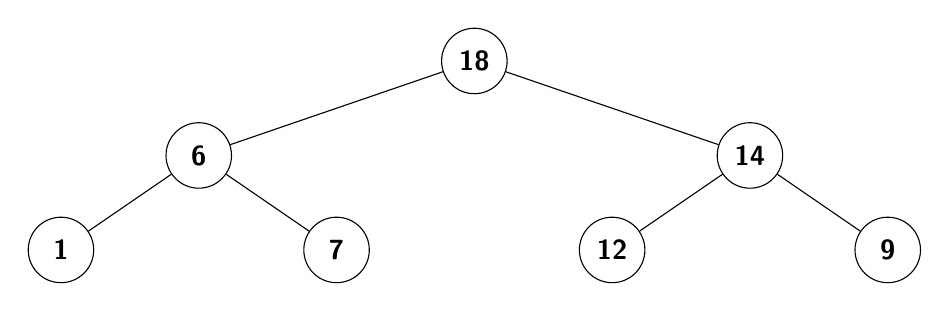
\begin{tikzpicture}[  treenode/.style = {align=center, inner sep=1pt, text centered,
    font=\sffamily},
  bst/.style = {treenode, circle, black, font=\sffamily\bfseries, draw=black, text width=2em}, 
  sst/.style = {treenode, circle, black, font=\sffamily\bfseries, draw=red, text width=2em}, 
  txt/.style = {text width=1.5em, red},
  redline/.style={edge from parent/.style={red,very thick,latex-, draw}},
  rugularline/.style={edge from parent/.style={black, line width=0.2mm, draw}},
  noline/.style={edge from parent/.style={black, line width=0.2mm}},
  level/.style={sibling distance = 7cm/#1,
  level distance = 1.2cm}
  ]
  \node [bst] (2n1) {18}
  child {node [bst] {6}
      child {node [bst] {1}
      }
      child {node [bst] {7}
      }
  }
  child { node [bst] {14}
      child{node [bst] {12}}
      child{node [bst] {9}}
  }
;
\end{tikzpicture}

\end{frame}

{
    % \usebackgroundtemplate{\transparent{0.3}{\begin{picture}
    %     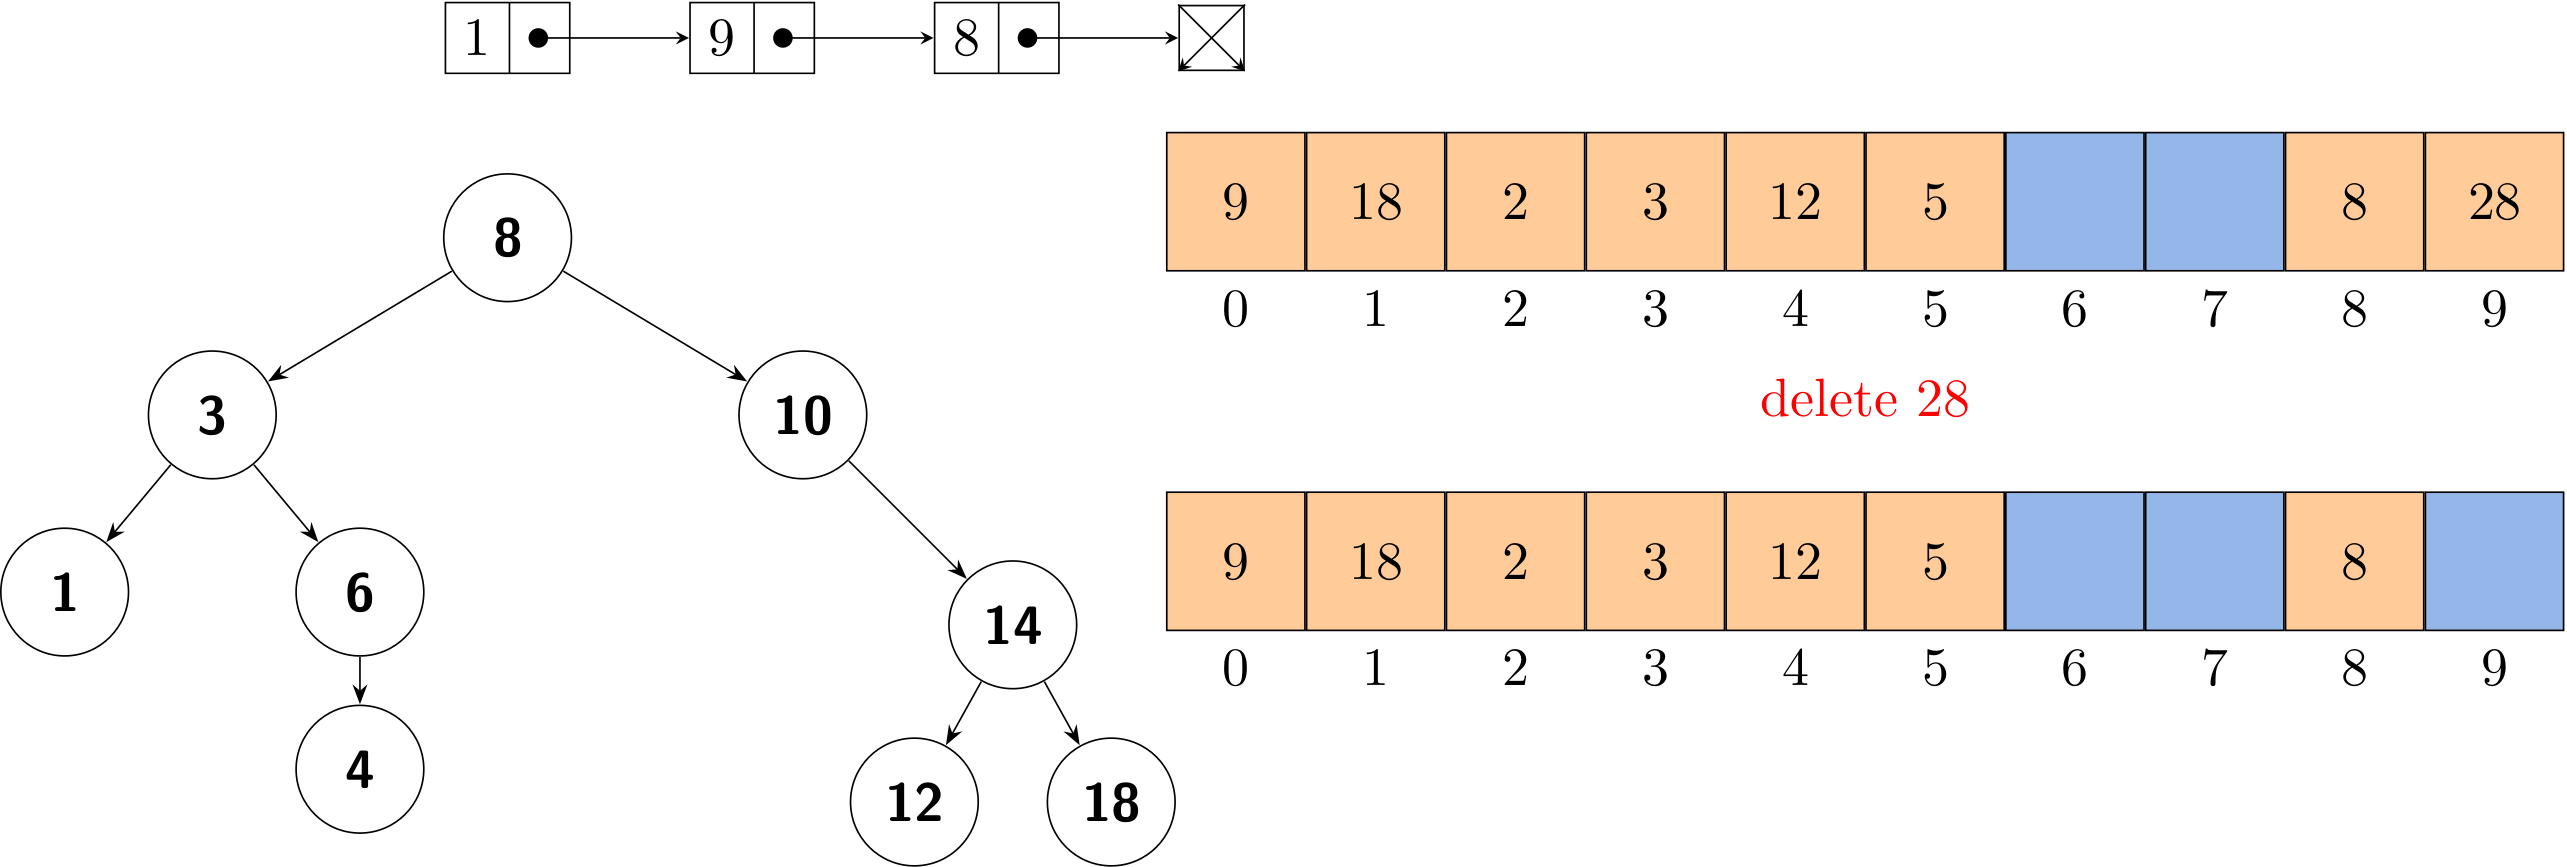
\includegraphics[height=0.7\paperheight]{cover}
    % \end{picture}    
    % }}
\usebackgroundtemplate{
  \tikz[overlay,remember picture] 
  \node[opacity=0.3, at=(current page.south east),anchor=south east, yshift=2cm,xshift=4cm] {
    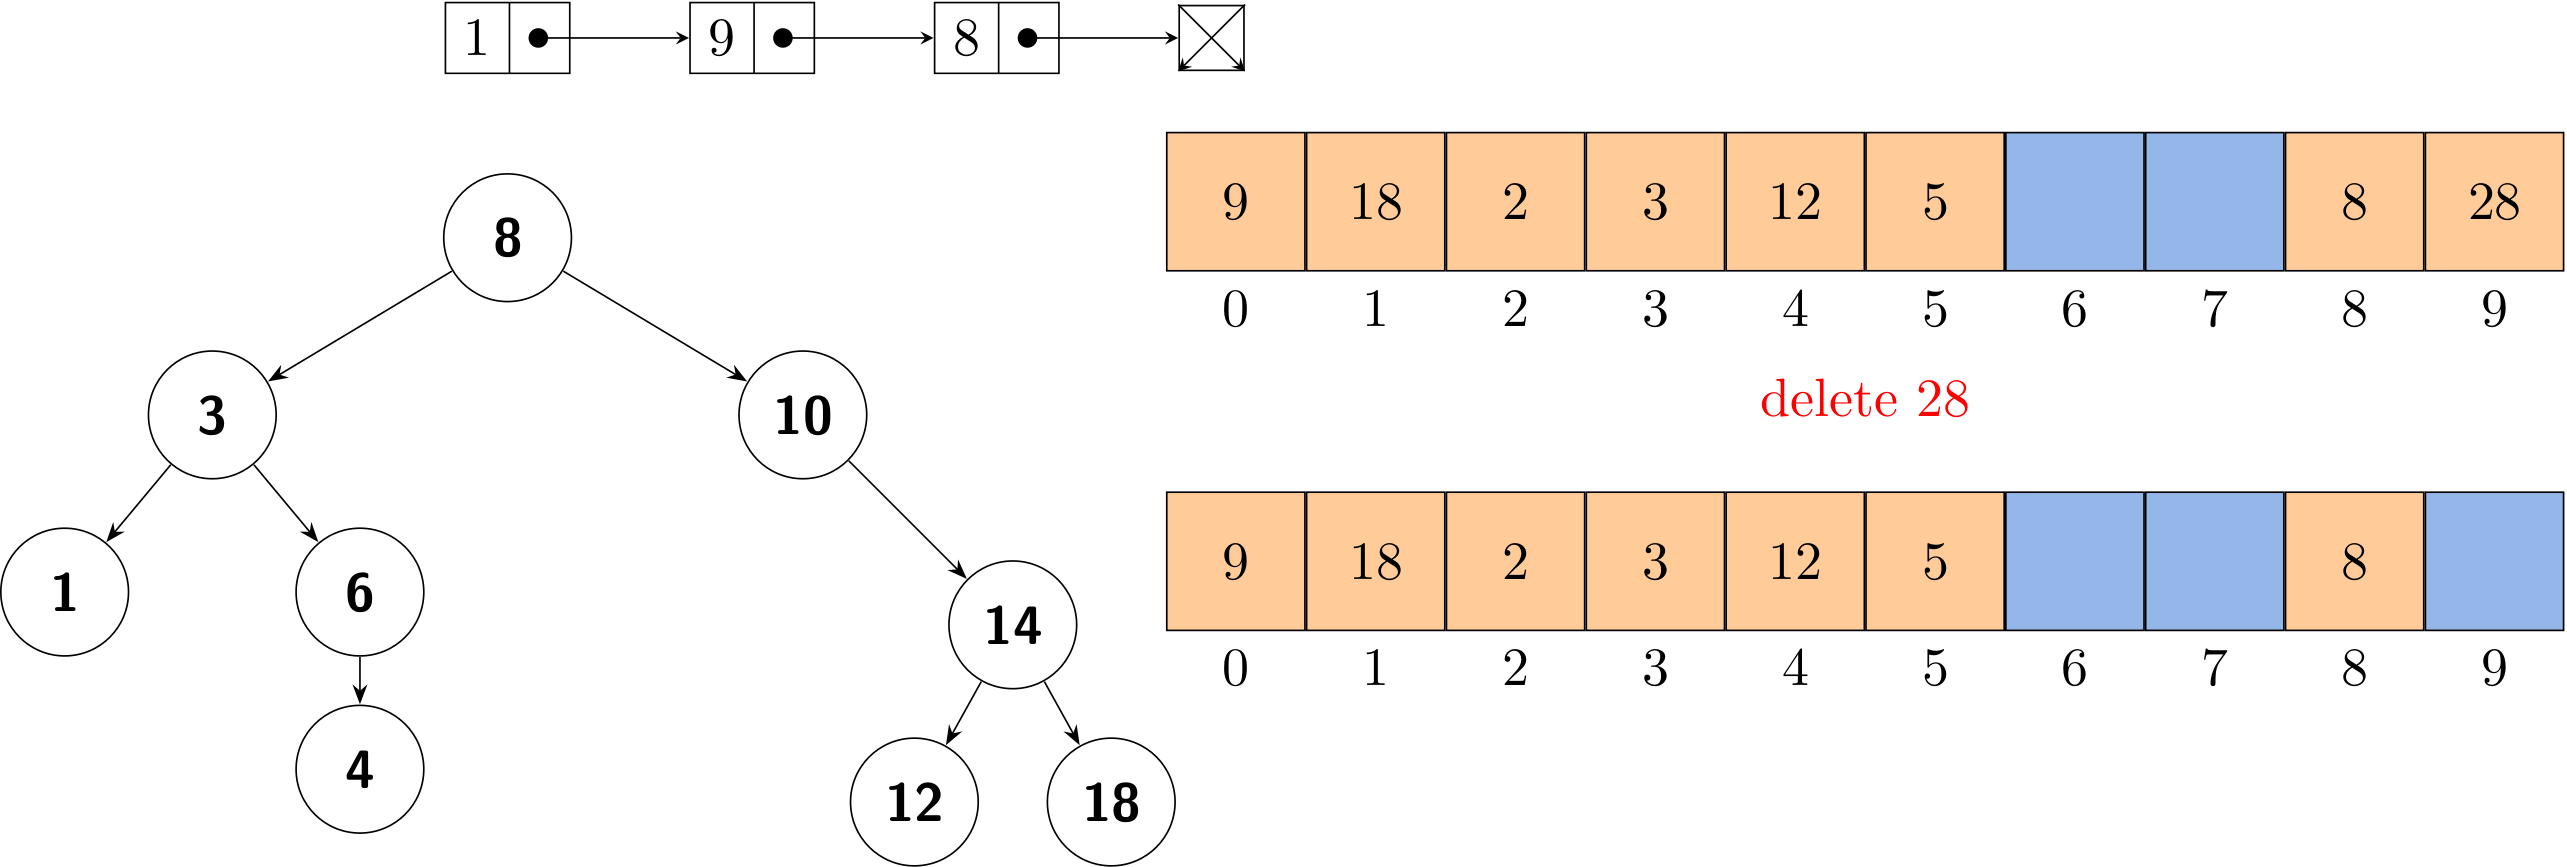
\includegraphics[height=0.6\paperheight]{cover}};
}
    \begin{frame}
        \section{\textcolor{darkmidnightblue}{1. From Arrays to Hashing}}
    \end{frame}

}
\begin{frame}[fragile]
    \frametitle{1.1 Motivation}

    \begin{block}{Fill in the blank}
    \faIcon{code} (Fill in the blank using big O notation.) Given an array, we can access an element by its index in \rule{1cm}{0.15mm} time.        
    \end{block}

    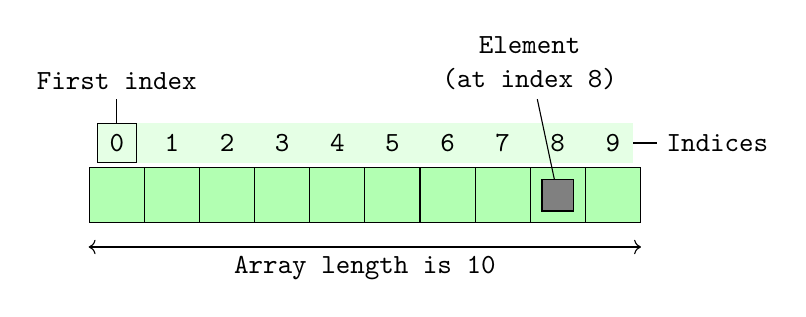
\begin{tikzpicture}[font=\ttfamily,
        array/.style={matrix of nodes,nodes={draw, minimum size=7mm, fill=green!30},column sep=-\pgflinewidth, row sep=0.5mm, nodes in empty cells,
        row 1/.style={nodes={draw=none, fill=none, minimum size=5mm}},
        row 1 column 1/.style={nodes={draw}}}]
        
        \matrix[array] (array) {
        0 & 1 & 2 & 3 & 4 & 5 & 6 & 7 & 8 & 9\\
          &   &   &   &   &   &   &   &   &  \\};
        \node[draw, fill=gray, minimum size=4mm] at (array-2-9) (box) {};
        
        \begin{scope}[on background layer]
        \fill[green!10] (array-1-1.north west) rectangle (array-1-10.south east);
        \end{scope}
        
        \draw[<->]([yshift=-3mm]array-2-1.south west) -- node[below] {Array length is 10} ([yshift=-3mm]array-2-10.south east);
        
        \draw (array-1-1.north)--++(90:3mm) node [above] (first) {First index};
        \draw (array-1-10.east)--++(0:3mm) node [right]{Indices};
        \node [align=center, anchor=south] at (array-2-9.north west|-first.south) (8) {Element\\ (at index 8)};
        \draw (8)--(box);
    \end{tikzpicture}

\end{frame}

\begin{frame}[fragile]
    \frametitle{Let's Play Games}
Suppose you are the CTO of an online cards game company, how do you design a data structure to store those cards?

    \crdtwoh \crdeigh \crdtred \crdtrec \crdfivec \crdfivec

It should be able to perform \alert{search()}, \alert{delete()}, and \alert{insert()} efficiently. Note that only cards with numbers are considered in the game.

\end{frame}

\begin{frame}[fragile]

    \begin{minted}[bgcolor=LightGray, baselinestretch=1.1]{python}
cards1 = [2, 8, 3, 3, 5, 5]

cards2 = [0, 1, 1, 0, 1, 0, 0, 1, 0, 0]
    \end{minted}

    \textbf{\faIcon{eye} View arrays from another perspective}: As for an array, the \alert{index} is the \textbf{key}, and the stored element is the \textbf{value}. 
    
    \begin{exampleblock}{Set and Map}
To manage these keys, we need a dynamic \alert{set}. If values (i.e., satellite data) are also kept, it is in fact a \alert{map} (i.e., dictionary).
    \end{exampleblock}

\end{frame}



\begin{frame}[fragile]
    \frametitle{1.2 Direct-address Table}

\begin{columns}
    \column{.65\textwidth}

    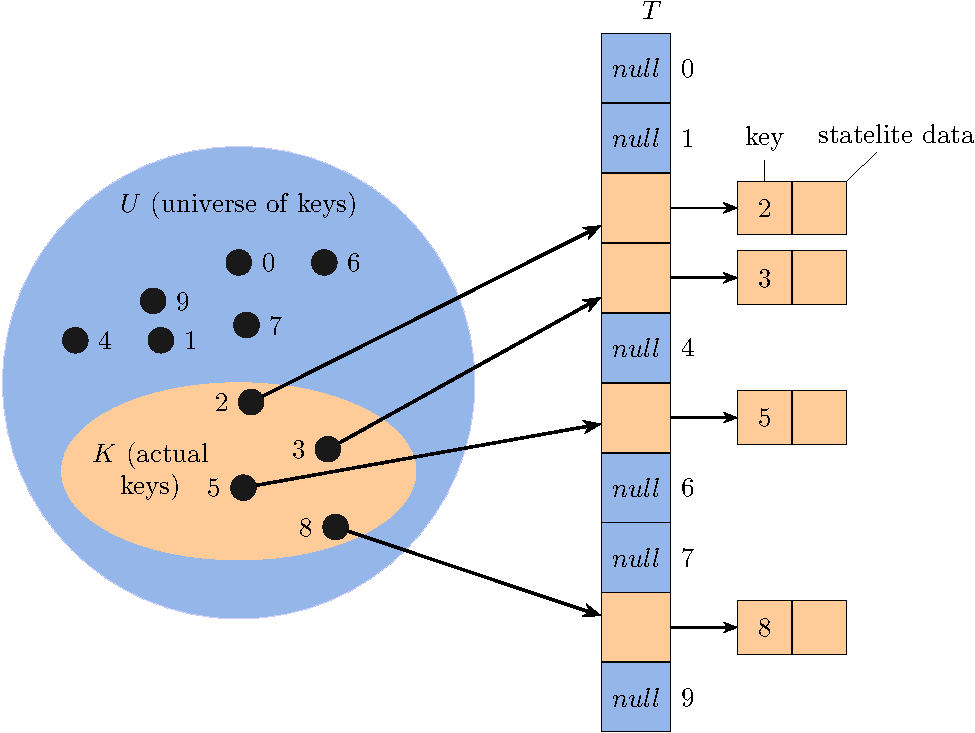
\includegraphics[width=.98\textwidth]{week11/direct}
    \column{.35\textwidth}
    Suppose each element has distinct key drawn from the universe $U = \{0, 1, \dots, m - 1\}$, where $m$ is not too large. In this case, an array is also known as a \alert{direct-address table}.
\end{columns}

\end{frame}

\begin{frame}
    \frametitle{Pitfalls of Direct-address Table}

    \begin{itemize}
        \item If the universe $U$ is large or infinite, storing a table $T$ may be impractical, or even impossible.
        \item Keys can only be integers.
    \end{itemize}
\end{frame}

\begin{frame}[fragile]
    \frametitle{1.3 Built-in Set and Map}
\faIcon{java} In Java, you can use \href{https://docs.oracle.com/en/java/javase/11/docs/api/java.base/java/util/HashSet.html}{HashSet} and \href{https://docs.oracle.com/en/java/javase/11/docs/api/java.base/java/util/HashMap.html}{HashMap}. While in Python, you can use \texttt{set} and \texttt{dict}. 

\begin{minted}[bgcolor=LightGray, baselinestretch=1.1]{python}
cards = {2, 8, 3, 5}  # set

cards_dict = {2: 1, 3: 2, 5: 2, 8: 1}  # dict
\end{minted}

The solution to pitfalls of a direct-address table is \alert{hashing}. Indeed, the built-in dictionaries of Python are implemented with hash tables.

\end{frame}

\begin{frame}

    \section{\textcolor{darkmidnightblue}{2. Hashing Tables}}
\end{frame}

\begin{frame}
    \frametitle{2.1 Hashing}
\begin{exampleblock}{Hash Function}
The hash function $h$ maps the universe $U$ of keys into the slots of a \alert{hash table} $T[0:m-1]$:   

\[h: U \rightarrow \{0, 1, \dots, m - 1\}\]

where the size $m$ of the hash table is typically much less than $|U|$.
\end{exampleblock}
    
A simple, but not particularly good, hash function is $h(k) = k \ mod \ m$.
\end{frame}

\begin{frame}
\begin{columns}
    \column{.65\textwidth}
    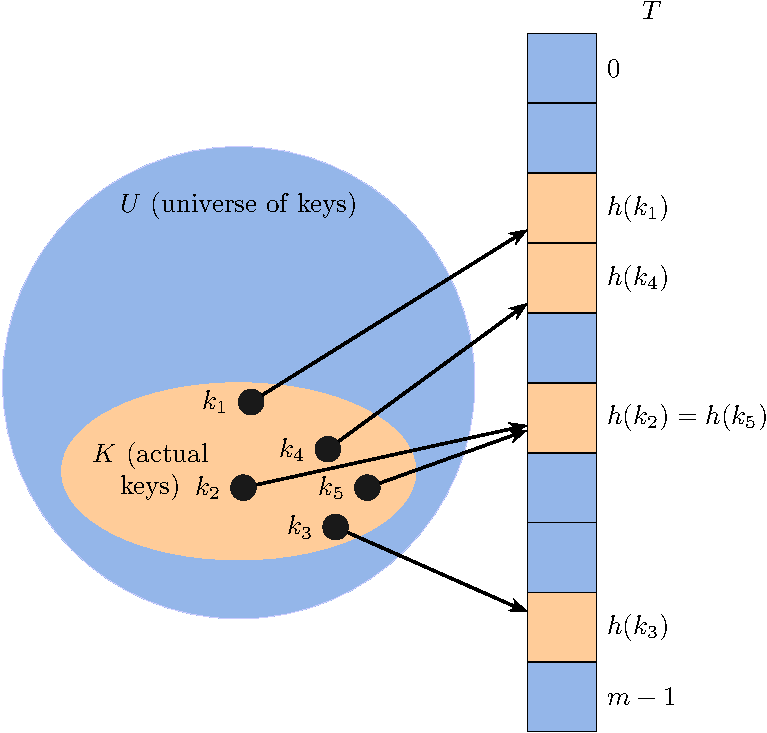
\includegraphics[width=.95\textwidth]{week11/table}
    \column{.35\textwidth}
    \faIcon{envira} \textbf{Two major issues}
    \begin{itemize}
        \item Design good hash functions
        \item Resolve collisions
    \end{itemize}
\end{columns}


\end{frame}

\begin{frame}
    \frametitle{2.2 Collision Resolution: Separate Chaining}
Suppose we adopt $h(k) = k \ mod \ m$, where $m = 10$. 

\begin{exampleblock}{Chaining}
    Each nonempty slot points to a linked list, and all the elements that hash to the same slot go into that slot's linked list.
\end{exampleblock} 
    
\sout{Note that in practice data structures that store the separate chains are not limited to a linked list, other data structures (e.g., a resizing array, a red-black tree) are also feasible.}
\end{frame}

\begin{frame}    
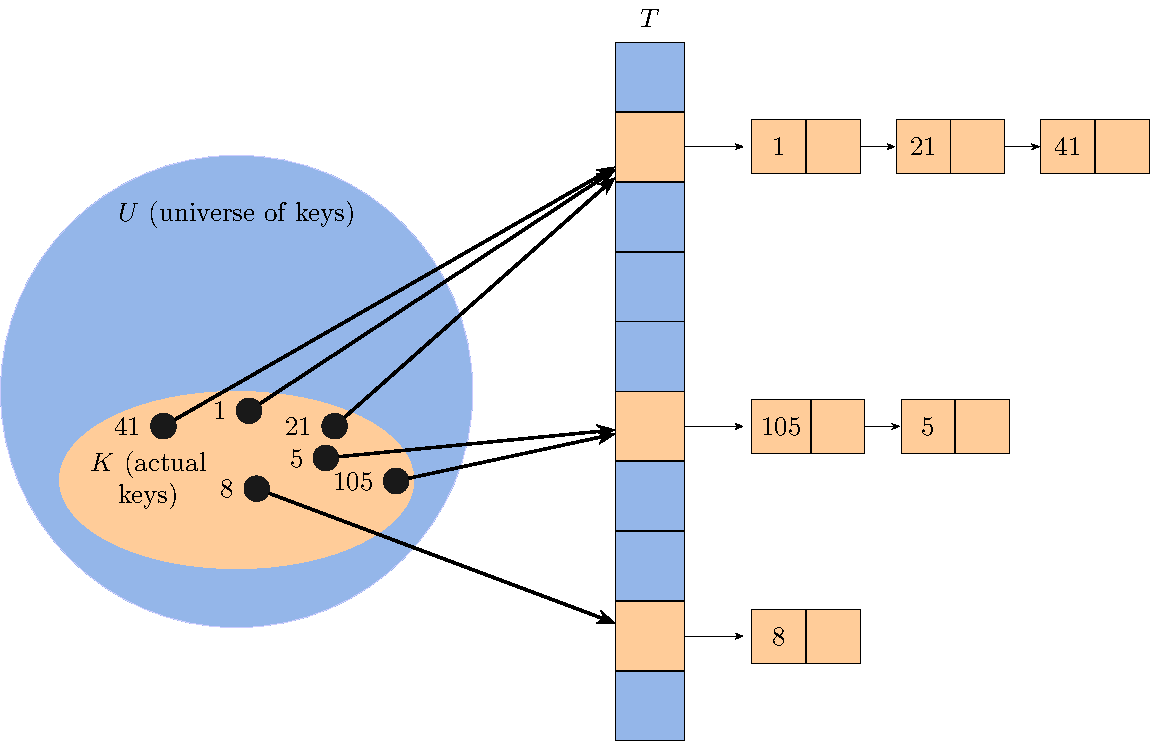
\includegraphics[width=.85\textwidth]{week11/chain}
\end{frame}

\begin{frame}
    \frametitle{Analysis}

\begin{exampleblock}{Uniform Hashing Assumption}
The hash functions that we use uniformly and independently distribute keys among the integers values between $0$ and $M - 1$.    
\end{exampleblock}

    Given a hash table $T$ with $m$ slots that stores $n$ elements, we define \alert{load factor} $\alpha$ for $T$ as $n/m$, that is, \textbf{the average number of elements stored in a chain}.

    \begin{exampleblock}{Theorem}
Under the Assumption above, a search takes $O(1+\alpha)$ time on average.        
    \end{exampleblock}
\end{frame}

\begin{frame}[fragile]
    \frametitle{Pseudo code}
The hash table $T$ maintains an array of linked lists.

\scalebox{.8}{
    \begin{algorithm}[H]
        \caption*{chained\_hash\_search(k)}
        \Return{T[h(k)].search(k)}
    \end{algorithm}
}

\scalebox{.8}{
    \begin{algorithm}[H]
        \caption*{chained\_hash\_insert(x)}
        T[h(x.key)].insert(x)
    \end{algorithm}
}

\scalebox{.8}{
    \begin{algorithm}[H]
        \caption*{chained\_hash\_delete(k)}
        T[h(k)].delete(k)
    \end{algorithm}
}
\end{frame}

\begin{frame}
    \frametitle{Re-hashing}
\faIcon{lightbulb} What if the load factor $\alpha$ becomes too large?
    
The solution is to resize the array, and then \alert{re-hashing}.

\par\noindent\rule{\textwidth}{0.4pt}

\faIcon{book-reader} Please read \href{https://github.com/ChenZhongPu/data-structure-swufe/blob/master/code/python/hash/separate_chaining_hash.py}{separate\_chaining\_hash.py}, and the code about how to use it can be found at \href{https://github.com/ChenZhongPu/data-structure-swufe/blob/master/code/python/hash/test_separate_chaining_hash.py}{test\_separate\_chaining\_hash.py}. Do you have any question?

\end{frame}

\begin{frame}
    \frametitle{2.3 Open-addressing Hash}
If we store $n$ elements in a hash table of size $m > n$, then it is called \alert{open-addressing} hash method. \textbf{All elements are stored in the hash table itself}.

\begin{block}{Collision Resolution}
With this method a hash collision is resolved by \alert{probing}, or searching through to find the next empty slot.
\end{block}

\end{frame}

\begin{frame}
    \frametitle{Linear Probing}
Suppose $h(k) = k \ mod \ m$, where $m = 10$:
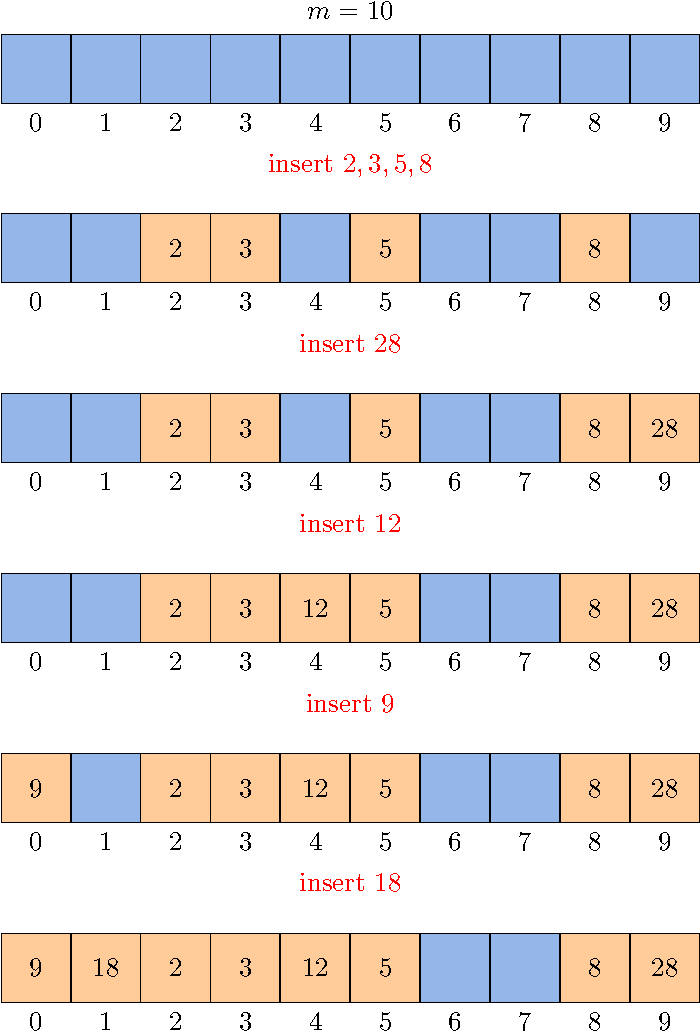
\includegraphics[width=.7\textwidth, trim={0 12cm 0 0},clip]{week11/probe}

\end{frame}

\begin{frame}
    \frametitle{Linear Probing (Cont.)}
    It always finds the \textbf{next} empty slot \alert{linearly} (in which the interval between probes is fixed, often set to 1.):
    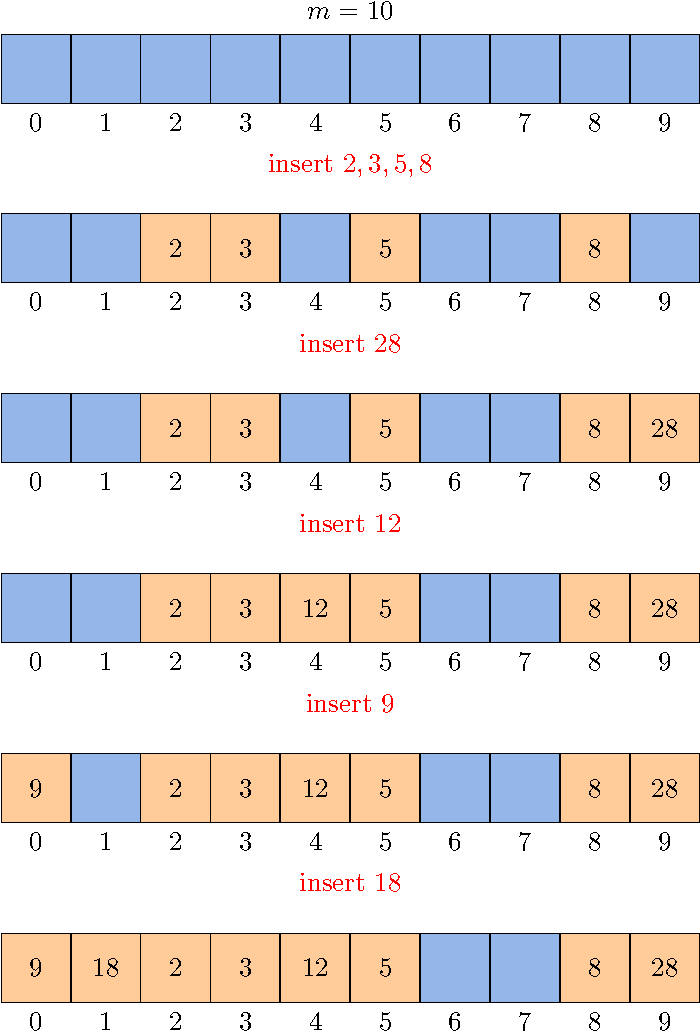
\includegraphics[width=.7\textwidth, trim={0 9cm 0 5.5cm},clip]{week11/probe}

\faIcon{pen} Please draw the result after inserting 12, 9, and 10.
\end{frame}

\begin{frame}[fragile]
    \frametitle{Search}

    \scalebox{.8}{
        \begin{algorithm}[H]
            \caption{hash-search(k)}
            \KwIn{The key $k$}
            \KwOut{The associated value of $k$}
            $i\gets 0$ \\
            \Repeat{keys[q] = null or i = m}{
                $q\gets h(k, i)$ \tcp{$h(k, i) = (h(k) + i) \ mod \ m$}
                \If{T[q].key == k}{
                    \Return{T[q].value}
                }
                $i\gets i + 1$
            }
            \Return{null}
        \end{algorithm}        
    }

\end{frame}

{\setbeamercolor{palette primary}{fg=black, bg=yellow}
\begin{frame}[standout]
  Open-addressing is also called closed hashing.
\end{frame}
}

\begin{frame}
    \frametitle{Other Probing}

    \begin{itemize}
        \item Quadratic probing: $h(k, i) = (h(k) + i + i^2) \ mod \ m$
        \item Double hashing: $h(k, i) = (h_1(k) + i \times h_2(k)) \ mod \ m$
    \end{itemize}

\end{frame}

\begin{frame}

    \section{\textcolor{darkmidnightblue}{3. Hashing Functions}}

    \begin{exampleblock}{Uniform Hashing Assumption}
        The hash functions that we use uniformly and independently distribute keys among the integers values between $0$ and $M - 1$.    
    \end{exampleblock}

\end{frame}

\begin{frame}
    \frametitle{3.1 Self-defined Hash Functions}

    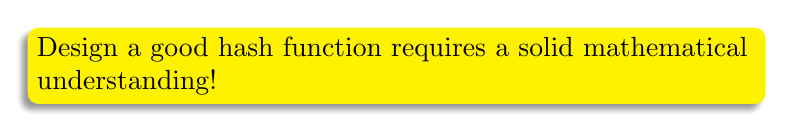
\begin{tikzpicture}
        \node[fill=yellow,blur shadow={shadow xshift=-0.5ex},
        text width=26em,anchor=south west,rounded corners]
        {Design a good hash function requires a solid mathematical understanding!};
    \end{tikzpicture}

    It is common to view the evaluation of a hash function, $h(k)$, as consisting of two parts:
\begin{itemize}
    \item a \textbf{hash code} that maps a key k to an integer
    \item a \textbf{compression function} that maps the hash code to an integer within a range of slots
\end{itemize}

\end{frame}

\begin{frame}
    \frametitle{Hash Code Of String}
As for character strings that can be viewed as tuples of the form $(x_0, x_1, \dots, x_{n-1})$, we choose a non-zero constant a ($\neq 1$) to compute its hash code:
    
\[x_0a^{n-1} + x_1a^{n-2} + \dots + x_{n-2}a + x_{n-1} \]

This method is also known as \alert{polynomial hash code}.
\end{frame}

\begin{frame}[fragile]
    \frametitle{Hash Code of Compound Keys}
If the key type has multiple fields, we can typically mix them together in the way just described for \texttt{String} values.

\begin{minted}[bgcolor=LightGray, baselinestretch=1]{java}
class PhoneNumber {
    private short areaCode;
    private short prefix;
    private short lineNum;
    ...
}    
\end{minted}
\[(31 \times areaCode + prefix) \times 31 + lineNum \]
\end{frame}

\begin{frame}[fragile]
    \frametitle{Exercise}
How to compute a hash code for the following class?
    
\begin{minted}[bgcolor=LightGray, baselinestretch=1.2]{java}
class Dog {
    private String name;
    private int age;
    ...
}    
\end{minted}

\end{frame}

\begin{frame}[fragile]
    \frametitle{3.2 Built-in Hash Code}
Java has already provided built-in feasible implementations for common data types:

\begin{minted}[bgcolor=LightGray, baselinestretch=1]{java}
Float.hashCode(3.14f);
String.hashCode("hello");
\end{minted}
As for multiple fields, you can even use \texttt{hash()} method:
\begin{minted}[bgcolor=LightGray, baselinestretch=1]{java}
@Override
public int hashCode() {
    return Objects.hash(name, age);
}
\end{minted}

\end{frame}

\begin{frame}[fragile]
    \frametitle{Built-in Hash Code}

    \begin{minted}[bgcolor=LightGray, baselinestretch=1]{python}
class Book:
    def __init__(self, name, price):
        self._name = name
        self._price = price

    def __hash__(self):
        return hash((self._name, self._price))
    \end{minted}

\end{frame}

\begin{frame}

    \section{\textcolor{darkmidnightblue}{Conclusion}}
    \begin{itemize}
        \item Hashing functions
        \item Separate chaining
        \item Linear probing (open-addressing)
    \end{itemize}
\end{frame}

\end{document}